%
% Copyright (c) 2020 Antonio Coín Castro
%
% This work is licensed under a
% Creative Commons Attribution-ShareAlike 4.0 International License.
%
% You should have received a copy of the license along with this
% work. If not, see <http://creativecommons.org/licenses/by-sa/4.0/>.

Having presented ordinary differential equations and their solutions in the previous chapter, we now focus on our main goal: the study and understanding of \textit{implicit} differential equations, that is, equations which are not solved for the derivative $y'$. Since we cannot put this type of equations into explicit form, all the theory discussed earlier does not apply directly to this case, and thus we want to find a general framework that allows for the treatment of these equations from a theoretical point of view. For this task we will refer to \cite[\S \ 25]{petrovski1966ordinary} and \cite[\S \ 3]{arnold2012geometrical}.

Given that equations are expressed in the general or implicit form, it makes sense to think that the \textit{implicit function theorem} will play a significant role in disentangling the complexities behind this formulation of differential equations, and that it will tell us something about their local behaviour. In an effort to provide all the necessary tools for the study we are about to undertake, we write down the statement of this famous theorem below.

\begin{theorem}[Implicit function theorem]
Let $D$ be an open set in $\R^{n+m}$ with coordinates $(x, y)$ and let $F:D \to \R^m$ be continuously differentiable. If $(a,b)\in D$ verifies $F(a,b)=0$ and the Jacobian matrix $\frac{\partial F}{\partial y}(a, b)$ is non-singular, then there exists an open set $U \subset \R^n$ with $a \in U$ and a unique $\mathcal C^1$ function $f:U\to \R^m$ such that:
\begin{enumerate}
  \item $f(a)=b$.
  \item $F(x, f(x)) = 0$ for all $x$ in $U$.
  \item The Jacobian matrix of $f$ is given by the matrix product
  \[
    Jf(x) = - \left( \frac{\partial F}{\partial y}(x, f(x))\right)^{-1} \left( \frac{\partial F}{\partial x}(x, f(x)) \right), \quad x \in U.
  \]
\end{enumerate}
\end{theorem}

\begin{proof}
A standard proof employing the equally renowned inverse function theorem can be found in \cite[374]{apostol1974analysis}. The last differentiation formula is obtained by differentiating the expression $F(x,f(x)) = 0$ and applying the chain rule.
\end{proof}

Even though we have stated the theorem for arbitrary dimensions, we will only apply it when $n=2$ and $m=1$, making the Jacobian matrix a single partial derivative. In fact, we recover the notation established in the previous chapter, and henceforth consider a function $F:\R^3 \to \R$ in $(x,y,p)$-space and the associated differential equation
\begin{equation}\label{eq:ode-implicit}
  F(x,y,y') = 0.
\end{equation}
Also, following a standard notation, we will denote by $F_x$, $F_y$ and $F_p$ the partial derivatives of the function $F$ with respect to each of its three variables $x$, $y$ and $p$. Then, the theorem assumes the following form:

\begin{corollary} \label{cor:implicit}
  Let $D$ be an open subset of $\R^3$ and let $F:D \to \R$ be continuously differentiable. If $(x_0, y_0, p_0) \in D$ verifies $F(x_0, y_0, p_0) = 0$ and $F_p(x_0,y_0,p_0) \neq 0$, then there exists an open set $U\subset \R^2$ containing $(x_0, y_0)$ and a unique $\mathcal C^1$ function $f:U\to \R$ such that $p_0=f(x_0,y_0)$ and $F(x, y, f(x,y))=0$ for all $(x, y) \in U$. Moreover, the partial derivative of $f$ with respect to its second variable is given by
  \begin{equation} \label{eq:der-formula}
  \frac{\partial f}{\partial y}(x, y) = - \frac{F_y(x,y, f(x,y))}{F_p(x, y, f(x,y))}.
\end{equation}
\end{corollary}

\section{Integral curves of implicit equations}

In this case we will start with an example. If we consider the differential equation
\begin{equation} \label{eq:ex1}
  (y')^2 = y,
\end{equation}
we should immediately observe that this expression is an abbreviation for two distinct explicit differential equations: $y'=\sqrt y$ and $y'=-\sqrt y$, for $y > 0$. Each of these equations produces a direction field, as seen in Figure \ref{fig:ex1}, and each of them separately satisfies an existence and uniqueness theorem on its domain, though clearly the uniqueness of solution fails when combining them. Nevertheless, we would like to examine this kind of equations as a whole, and establish general conditions for their treatment.

\begin{figure}[h!]
\centering
\begin{subfigure}{.6\textwidth}
  \centering
  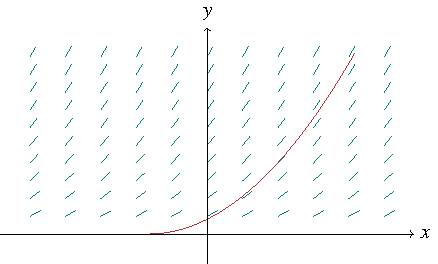
\includegraphics[width=\linewidth]{ex1}
\end{subfigure}
\begin{subfigure}{.6\textwidth}
  \centering
  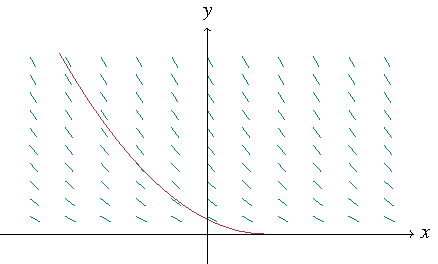
\includegraphics[width=\linewidth]{ex2}
\end{subfigure}
\caption{Direction fields of the two equations combined in the notation $(y')^2=y$.}
\label{fig:ex1}
\end{figure}

One thing to note from the beginning is that there are some occasions in which implicit equations can be put in explicit form, at least in theory. That is, there is a set of conditions that, when satisfied, guarantee that the equation is equivalent to another one in explicit form. Of course, in non-trivial cases this result will only hold locally, and as one would expect it is a direct consequence of the aforementioned implicit function theorem.

\begin{theorem} \label{th:implicit-basic}
  Let $F:D \to \R$ be a continuously differentiable function on some domain $D$ of the $(x,y,p)$-space. Suppose that $(x_0,y_0,p_0) \in D$ simultaneously satisfies $F(x_0,y_0,p_0)=0$ and $F_p(x_0,y_0,p_0)\neq 0$. Then there exists a unique function $\phi$ defined on an interval containing $x_0$ that is a solution of the equation $F(x,y,y')=0$, satisfying $\phi(x_0)=y_0$ and $\phi'(x_0)=p_0$.
\end{theorem}

\begin{proof} Under these conditions we can apply Corollary \ref{cor:implicit} to $F(x,y,p)$ and express $p$ as a function of $x$ and $y$, that is, there exists a unique smooth $f$ such that $F(x,y,f(x,y))=0$ on a neighbourhood $U$ of the point $(x_0,y_0)$, that also verifies $p_0=f(x_0,y_0)$. Then the IVP
\[
  \begin{cases} y' = f(x,y) & \text{in } U,\\
    y(x_0)=y_0
  \end{cases}
\]
is well defined, and since $f_y$ is continuous, it verifies the conditions of Theorem \ref{th:picard}. Thus, there is a unique smooth function $\phi$ defined on a neighbourhood $I$ of $x_0$ such that $\phi'(x)=f(x, \phi(x))$ on $I$ and $\phi(x_0)=y_0$. This concludes the proof, seeing as how putting it all together we have
\[
p_0 = f(x_0, y_0) = f(x_0, \phi(x_0)) = \phi'(x_0)
\]
and
\[
F(x,\phi(x), \phi'(x)) = F(x, \phi(x), f(x, \phi(x))) = 0, \quad x \in I.
\]

\end{proof}

\begin{remark} Uniqueness of solution may fail if the requirement that $F_p\neq 0$ is not satisfied. For example, consider the equation
\[
(y')^2 - 2y' + 4y - 4x + 1 = 0,
\]
for which at the point $(0,0,1)$ we have $F_p=0$ but both $x$ and $x-x^2$ are valid solutions that satisfy the initial conditions.
\end{remark}

If we take a closer look at the above result, we observe that for every choice of $p_0$ there is a potentially different solution to the equation. But just how many suitable points are there? Is there any condition that guarantees that the number of possible solutions passing through a given point in the plane is finite? The following theorem (cf. \cite[76]{petrovski1966ordinary}) gives a satisfactory answer, namely that we can limit the number of solutions in a neighbourhood if after setting a reference point $(x,y)$ we can solve the (algebraic) equation for $p$.

\begin{theorem} \label{th:implicit2} Let $F:D \to \R$ be a continuous function defined on some domain $D \subset \R^3$ with coordinates $(x,y,p)$. Suppose that $(x_0,y_0) \in \R^2$ is such that the equation $F(x_0,y_0,p)=0$ has a finite number of distinct roots $p_1,\dots, p_m$ when solved for $p$, verifying that $(x_0,y_0,p_i) \in D$ and that $F_p(x_0,y_0,pi) \neq 0$ for $i=1,\dots,m$. Further suppose that for $i=1,\dots,m$ there exists a neighbourhood $\mathcal R_i$ of the point $(x_0,y_0,p_i)$ in which $F$ is continuously differentiable. Then there is a neighbourhood $\mathcal N$ of $(x_0,y_0)$ such that precisely $m$ solutions of the equation
  \begin{equation} \label{eq:implicit-th}
  F(x,y,y')=0
\end{equation}
  pass through each point of $\mathcal N$.

\end{theorem}

\begin{proof}

Since the set $\{p_1,\dots,p_m\}$ is finite, we can suppose without loss of generality that the $\mathcal R_i$ are cylinders parallel to the $p$-axis, where the projection of the base of each cylinder onto the $(x,y)$-plane is the same neighbourhood $\mathcal N$ of $(x_0,y_0)$, as shown schematically in Figure \ref{fig:cylinder}. This can be done, eventually shrinking the neighbourhoods, because they all enclose the same point $(x_0,y_0)$ in the $(x,y)$-plane. More precisely, there exist $r>0$ and $\epsilon > 0$ such that
\[
\mathcal R_i = B_r(x_0,y_0) \times (p_i-\epsilon, p_i+\epsilon), \quad i=1,\dots,m.
\]
In addition, we can choose $\epsilon$ sufficiently small so that
\begin{itemize}
  \item The cylinders are disjoint, that is, $\mathcal R_i \cap \mathcal R_j =\emptyset$, $i\neq j$.
  \item For every $(x,y,p) \in \mathcal \bigcup_{i=1}^m \mathcal R_i$ we have $|F_p(x,y,p)| \ge c > 0$ (this follows from the continuity of $F_p$).
\end{itemize}
Next we take a compact set $G$ such that
\[
\bigcup_{i=1}^m \overbar{\mathcal R}_i \subset G \subset D,
\]
and we will henceforth work in $G$, denoting
\[
  \mathcal R = \bigcup_{i=1}^m \mathcal R_i.
\]

\begin{figure}[h!]
\centering
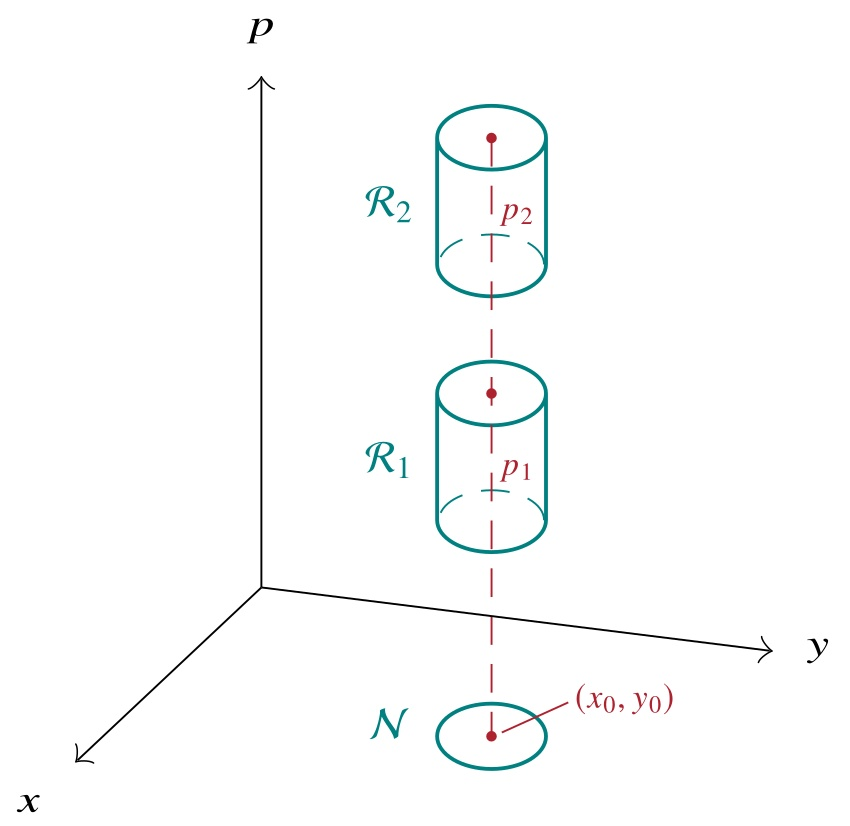
\includegraphics[width=.5\textwidth]{cylinder.jpg}
\caption{Representation of the cylindrical neighbourhoods of each $p_i$ and the projection of every base onto the $(x,y)$-plane.}
\label{fig:cylinder}
\end{figure}

In this situation the implicit function theorem asserts that in each of the cylinders $\mathcal R_i$ (shrunk if necessary) the equation  $F(x,y,p)=0$ is satisfied by one and only one choice of $p$ as a smooth function of $x$ and $y$, that is, of the form
\begin{equation}\label{eq:surface-th}
  p=f_i(x,y), \quad i=1,\dots,m,
\end{equation}
where in each case the derivative with respect to $y$ is given by \eqref{eq:der-formula}. Since $|F_p(x,y,f_i(x,y))| \ge c > 0$ by assumption and given that $F_y$ is continuous, we can assure that each $\partial f_i/\partial y$ is bounded on $\mathcal R_i$.

Not only that, but we can also choose $\mathcal N$ so small that every point $(x,y,p)$ in the cylinder generated by $\mathcal N$ for which $F=0$ belongs to one of the surfaces \eqref{eq:surface-th}. Indeed, if it were not the case, any such point would obviously have to lie outside the cylinders $\mathcal R_1, \dots, \mathcal R_m$, and if they existed for arbitrarily small $\mathcal N$ they would have to be on the line $x=x_0$, $y=y_0$. To see this, we argue by contradiction and suppose that for all $n \in \NN$ there exists a point $(x_n,y_n,p_n) \in G$ with the following properties:

\begin{enumerate}
  \item $F(x_n,y_n,p_n)=0$.
  \item $\lvert (x_n, y_n) - (x_0, y_0)\rvert < \frac{1}{n}$.
  \item $(x_n, y_n, p_n) \in G \setminus \mathcal R$.
\end{enumerate}
Since $G$ is compact, $\{p_n\}$ is bounded, and we can suppose that it converges to some real value $p_0$. Together with property $(ii)$, this information assures that
\[\{(x_n,y_n,p_n)\} \to (x_0,y_0,p_0).
\]
Now, since $G \setminus \mathcal R$ is closed in $G$, $(iii)$ implies that $(x_0,y_0,p_0) \notin \mathcal R$, and in particular that $p_0 \notin \{p_1,\dots,p_m\}$. Finally, by virtue of $(i)$ and the continuity of $F$, we conclude that
\[
0=F(x_n,y_n,p_n) \to F(x_0,y_0,p_0),
\]
meaning that $p_0$ is another root of the equation $F(x_0,y_0,p)=0$, which is impossible since its only roots were $p_1,\dots,p_m$.

Thus we have proven that the point $(x_0,y_0)$ has a neighbourhood $\mathcal N$ where $F(x,y,p)=0$ has precisely $m$ solutions \eqref{eq:surface-th}. Each function $f_i$ is continuous and has a bounded derivative with respect to $y$, so according to Theorem \ref{th:picard} each of the equations
\[
y' =f_i(x,y)
\]
has one and only one integral curve passing through any given point of $\mathcal N$. Repeating the reasoning in the proof of Theorem \ref{th:implicit-basic} we can see that these curves are indeed integral curves of \eqref{eq:implicit-th}. Because the values of $y'$ associated with each integral curve are all different on $\mathcal N$ (since the cylinders $\mathcal R_i$ are disjoint), these integral curves are all different and no two make contact without intersecting. Moreover, if there was another integral curve apart from these ones, its derivative would have to take the values $\overbar{p}_i \in \mathcal R_i$ and $\overbar{p}_j \in \mathcal R_j$ for some $i\neq j$, and by the \textit{intermediate value theorem for derivatives} (see footnote \ref{fn:darboux}) it would have to take every value in between, which is impossible since $F$ only vanishes on $\mathcal R$. Therefore, as asserted, precisely $m$ solutions of equation \eqref{eq:implicit-th} pass through each point of $\mathcal N$.
\end{proof}

A careful look at the statement of this problem reveals that none of the direction fields defined by equation \eqref{eq:implicit-th} can be parallel to the $y$-axis. However, as in the case of equations solved for $y'$, we would like to include this possibility. Therefore, besides the equation
\begin{equation}\label{eq:implicit-again}
  F\left(x,y,\frac{dy}{dx}\right)=0
\end{equation}
we consider the associated equation
\begin{equation}
  \tag{\ref*{eq:implicit-again}'}
  F_1\left(x,y,\frac{dx}{dy}\right)=0,
\end{equation}
where $F_1$ is chosen in such a way that these equations are consistent.

As a final remark, we note that if we could explicitly solve for $y'$ (think for example that $F$ were a polynomial on $y'$) then we could not only establish the existence and uniqueness of solutions, but also determine exactly what those solutions were, as in the next example.

\begin{example} \label{ex:parabolas} Let us revisit the equation
  \begin{equation} \label{eq:ex2}
    (y')^2=y.
  \end{equation}
We know that two direction fields are combined in this equation (see Figure \ref{fig:ex1}), and hence the direction field of \eqref{eq:ex2} is obtained as the superposition of those two direction fields. Setting $F(x,y,p)=p^2-y$ and solving $F=0$ for $p$ yields $p=\pm \sqrt{y}$, for every $y > 0$. We have $F_p=2p$, so we can apply Theorem \ref{th:implicit2} to every point on the set
\[
\{(x,y) \in \R^2: y > 0 \},
\]
obtaining that there is a neighbourhood of each of these points in which there are two and only two integral curves of equation \eqref{eq:ex2} passing through any given point. This is also obvious from Figure \ref{fig:ex1}. What is more, in this case we can obtain an explicit expression of those integral curves by solving the two differential equations
\begin{equation} \label{eq:parabolas}
y'= \pm \sqrt{y}, \quad y > 0,
\end{equation}
whose joint family of solutions can be written as
\[
y(x)=\frac{1}{4}(x+C)^2, \quad C \in \R.
\]
They are convex parabolas with vertex on the $x$-axis, the upwards branch corresponding to the positive sign in \eqref{eq:parabolas} and the downwards branch to the negative sign.
\end{example}

\begin{remark} The above example stresses the importance of working in open sets when it comes to uniqueness of solutions. If we were to solve equation \eqref{eq:ex2} for $y\ge 0$, we would immediately note that the line $y=0$ is an integral curve of the equation, and then an infinite number of solutions would pass through every point on the $x$-axis. In particular, for every $x_0 \in \R$ the functions parametrized by $k\ge x_0$ as
  \[
  \phi_k(x)= \begin{cases}
    0, & x < k,\\
    \frac{1}{4}(x-k)^2, & x \ge k
  \end{cases}
  \]
are all different solutions of the equation passing through the point $(x_0,0)$.

\end{remark}

\section{Geometrical approach to implicit equations}

When studying equations in implicit form, the previous results and techniques suggest a geometrical approach in which we consider the direction field not on the $(x,y)$-plane, but on the surface of the three-dimensional $(x,y,p)$-space given by the equation $F(x,y,p)=0$, where $p=dy/dx$. This way, even though the equation might define several direction fields, we compensate for this by adding a new dimension in which to visualize them together. This space is known as the space of \textit{1-jets} of functions $y(x)$, which is basically representing the truncated Taylor polynomial of a (differentiable) function at a given point. We can regard its points as all the non-vertical directions\footnote{We could circumvent this restriction with the usual trick of considering another function $F_1$, but we will not do it here for simplicity.} (those not parallel to the $y$-axis) at all points of the $(x,y)$-plane: a point $(x,y,p)$ represents the direction of a line $dy=p\,dx$ at the point $(x,y)$. In what follows, the direction of the $p$-axis will be referred to as the \textit{vertical direction} in the space of $1$-jets.

For the purposes of this section we will assume that $F$ is a sufficiently differentiable function and that the surface
\[
M = \{ (x,y,p) : F(x,y,p)=0\}
\]
in the space of 1-jets is smooth\footnote{This is not a strong restriction, since it holds if $0$ is not a critical value of $F$, and by Sard's theorem this happens almost always. Even if it were not the case, a small perturbation by an additive constant should make it so.}. We will show that a direction field arises on this surface and relate it to a certain direction field on the plane. Before we continue, we define a concept that will be essential in the development of the theory.

\begin{definition}
A point on the surface $M$ is called a \textit{regular point} if the tangent plane to the surface at that point is not vertical.
\end{definition}
Let us recall that the tangent plane at a point $(x_0,y_0,p_0)$ of the surface $M$ is given by the equation
\begin{equation} \label{eq:tangent}
\langle \nabla F(x_0,y_0,p_0), (x-x_0,y-y_0,p-p_0) \rangle = 0,
\end{equation}
so that it is non-vertical if and only if $F_p(x_0,y_0,p_0) \neq 0$. This condition should look familiar after seeing the results of the previous section. Let
\[
\pi:M\to\R^2, \quad \pi(x,y,p)=(x,y)
\]
be the projection of $M$ to the $(x,y)$-plane in the vertical direction. A \textit{critical point} of the mapping $\pi$ will be a point for which $F=F_p =0$, that is, a point on $M$ that is not regular.

Thus, in a neighbourhood of a regular point we can apply yet again the implicit function theorem to show that $M$ is the graph of a smooth function, say $p=f(x,y)$. In fact, it is a well-known result in the basic theory of differentiable surfaces that in this case the projection $\pi$ is a local diffeomorphism (see \cite[39]{montiel2009curves}). Then, to each regular point corresponds its own differential equation (in a neighbourhood of the projection of said point) and the direction field that comes with it; all these direction fields on the $(x,y)$-plane are combined in the equation $F=0$.

On the other hand, we forget the projection momentarily and consider a point $(x,y,p)$ in the space of 1-jets and a vector $\xi$ applied at this point, whose components will be denoted by $dx(\xi)$, $dy(\xi)$ and $dp(\xi)$. We now consider the plane of all such vectors at a point $(x,y,p)$ for which $dy=p\,dx$\footnote{In differential geometry this is known as (the kernel of) a 1-form.}, that is, the vectors that when projected onto the $(x,y)$-plane form an angle  with the $x$-axis whose tangent is equal to $p$. Each of these planes is called a \textit{contact plane}, and they are all vertical (they contain the direction of the $p$-axis, since the vector $(0,0,1)$ verifies the condition imposed). The set of all contact planes forms the \textit{contact plane field} in the space of jets, and is called the \textit{contact structure}\footnote{This term is not specific to this problem, but it is an important notion in a branch of geometry known as contact geometry, which falls outside of the scope of this work.}. Figure \ref{fig:jets} can help visualize the various elements of this construction.

\begin{figure}[h!]
\centering
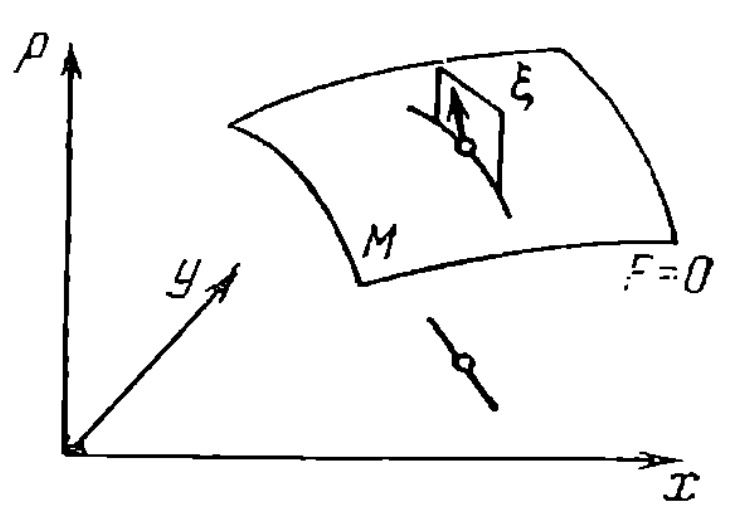
\includegraphics[width=.4\textwidth]{jets.jpg}
\caption{The surface $M$, the contact plane at a point and its projection. Taken from \cite{arnold2012geometrical}.}
\label{fig:jets}
\end{figure}

Bringing back the projection, we study the contact plane at a regular point of the surface $M$. Since the contact plane is vertical, it intersects the corresponding tangent plane in a line, and this behaviour is reproduced in all the nearby points. In this way, in a neighbourhood of a regular point there arises a smooth direction field, given by the intersections of the contact and tangent planes at every point. The integral curves of equation \eqref{eq:ode-implicit} are, by definition, the integral curves of this direction field on $M$. We can even provide an explicit description of this direction field by analyzing the intersection of the two planes. Firstly, since the contact plane at a regular point $(x,y,p)$ is given by the equation $p\,dx - dy = 0$, the normal vector to this plane at the point $(x,y,p)$ is $(p,-1,0)$, and secondly we know by equation \eqref{eq:tangent} that the normal vector to the tangent plane at said point is $\nabla F(x,y,p)$. Then, the line resulting from the intersection of both planes at the point of interest is given by the direction
\[
\nabla F(x,y,p) \times (p,-1,0) = {(F_p, pF_p, - (F_x+pF_y))\,}_{\mkern 1mu \vrule width 0.75pt height 2ex\mkern2mu \,(x,y,p)},
\]
and thus the direction field on $M$ is defined by the vector field
\begin{equation} \label{eq:field}
V = (F_p, pF_p, -(F_x+pF_y)).
\end{equation}

We are now ready to link these seemingly distinct direction fields (the one on $M$ and the ones on the $(x,y)$-plane we mentioned earlier), though it should be clear by now what the conclusion will be: that the direction field on $M$ projects locally onto a direction field on the plane.

\begin{theorem}
  The vertical projection onto the $(x,y)$-plane in the neighbourhood of a regular point maps integral curves of equation \eqref{eq:ode-implicit} on $M$ into integral curves of the equation
  \begin{equation} \label{eq:implicit-graph}
      \frac{dy}{dx}=f(x,y)
  \end{equation}
  in a neighbourhood of the projection of the point under consideration. Here $f$ is a smooth function such that $M$ is locally the graph of $f$.
\end{theorem}

\begin{proof}
We know by definition that the projection of a contact plane onto the $(x,y)$-plane is a straight line in the direction field of equation \eqref{eq:implicit-graph}, because it holds that $p=f(x,y)$. Then, since $\pi$ is a diffeomorphism in the neighbourhood considered, the direction field on $M$ turns into the direction field of \eqref{eq:implicit-graph}. Consequently, the integral curves turn into each other, as well.
\end{proof}

The conclusion we can extract from all this reasoning is that, in the neighbourhood of a regular point, an implicit equation can be turned into an explicit one and can be studied and solved with the usual methods. However, special attention should be paid to critical points, that is, points in which the equation does not reduce to an explicit one, and in fact we will expand on this matter in the next section. For now, we define a couple of concepts related to these points, and we bring this section to an end with an example.

\begin{definition} The set $C$ of critical points of the projection $\pi$ is called the \textit{criminant curve} of equation \eqref{eq:ode-implicit}, and the set $\pi(C)$ of its images is called the \textit{discriminant curve}.
\end{definition}

\begin{remark} The discriminant curve can be obtained in some cases by eliminating $p$ in the equations $F=F_p=0$.

\end{remark}

\begin{example} \label{ex:cusp}
  We want to study the equations $p^2=x$ and $p^2=y$ using the techniques of this section. For the first one, we write down the equations of a generic vector at a point $(x,y,p)$ on $M$ that belongs to the direction field:
  \[
  \begin{cases}
    p^2=x & \text{(the condition of belonging to $M$)},\\
    2p\,dp=dx & \text{(the condition of being tangent to $M$)},\\
    dy=p\,dx & \text{(the condition of belonging to the contact plane)}.
  \end{cases}
  \]
We note that the criminant is given by the curve $p=0$ on $M$, which results when projected in a discriminant curve consisting on the $x$-axis (it follows from the first condition that $x=0$ when $p=0$). In this case it is convenient to choose the coordinates $(p,y)$ on $M$. Combining the conditions above we get that (in our chosen coordinates) the integral curves are defined by the equation
\[
\frac{dy}{dp} = 2p^2,
\]
which we can easily solve to get that the solutions are given by the relation $y+C=\frac{2}{3}p^3$. Projecting back to the $(x,y)$-plane yields integral curves defined parametrically by
\[
x=p^2, \quad y= \frac{2}{3}p^3 + C, \quad C \in \R.
\]
If we want, we can also reverse the change of variables to write down the solutions as a more direct relation between $x$ and $y$:
\[
(y+C)^2 = \frac{4}{9}p^6 \implies (y+C)^2 = \frac{4}{9}x^3,\quad C \in \R.
\]
It can be checked that these solutions are semi-cubical parabolas with a cusp on the discriminant line $x=0$, as seen in Figure \ref{fig:parabola}.

\begin{figure}[h!]
\centering
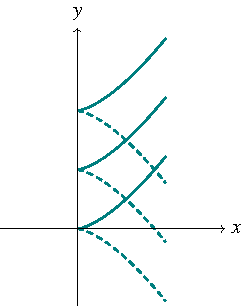
\includegraphics[height=17em]{parabola}
\caption{Integral curves of the equation $p^2=x$ on the plane.}
\label{fig:parabola}
\end{figure}

The other equation $p^2=y$ is solved in a similar way. The conditions in this case are the following:

  \[
  \begin{cases}
    p^2=y,\\
    2p\,dp=dy,\\
    dy=p\,dx.
  \end{cases}
  \]
The criminant is again $p=0$, but in this case the discriminant curve is the $x$-axis. If we choose coordinates $(x,p)$ on $M$ the resulting equation outside of the criminant is
\[
\frac{dx}{dp}=2,
\]
which yields solutions of the form
\[
x=2p + C, \quad y=p^2, \quad C \in \R,
\]
or equivalently,
\[
(x+C)^2=4y, \quad C \in \R.
\]
\end{example}
These are parabolas tangent to the line $y=0$, as we already knew from Example \ref{ex:parabolas}.

\section{Singular points and singular solutions}

Another common terminology for referring to the points on the criminant curve is to call them \textit{singular points} of the equation $F=0$. It is worth pointing out that at some singular points it may well be the case that the contact plane is different from the tangent plane, so that they intersect in a straight line and thus still produce a direction field. In fact, we can extend the direction field defined in the previous section to include these well-behaved points, and say that this extended field is the \textit{direction field of the equation $F=0$ on $M$}. However, at singular points the conditions to apply the implicit function theorem do not hold (we have $F_p=0$), so we can only assure that projections of the pieces of the integral curves (of the extended field) localized between singular points are locally integral curves of the corresponding equations $y'=f(x,y)$.

Following the distinction outlined above between singular points, and remembering the expression \eqref{eq:field} for the direction field on $M$, we arrive at the following definition.

\begin{definition}
  A singular point of equation $F=0$ (a point on $M$ for which $F_p=0$) is called a \textit{proper singular point} if $F_x+pF_y \neq 0$, and an \textit{improper singular point} otherwise.
\end{definition}
In the first case, if $(x_0,y_0,p_0)$ is a proper singular point, the tangent and contact planes intersect each other at the straight line passing through $(x_0,y_0,p_0)$ and having direction
\[
v=(0,0,-F_x(x_0,y_0,p_0)-p_0F_y(x_0,y_0,p_0)).
\]
In the second case, the contact and tangent planes coincide at the point $(x_0,y_0,p_0)$ and no straight line is produced. Now, among proper singular points we distinguish those which verify an additional smoothness condition: we will refer by \textit{regular singular point}\footnote{Not to be confused with a regular point of $\pi$.} or \textit{folded proper point} to a proper singular point that verifies
\[
\operatorname{rank}((x,y,p) \mapsto (F,F_p)) = 2,
\]
where the rank of a mapping is defined as the rank of its derivative (which is a linear map). Note that this condition guarantees via the implicit function theorem that the criminant curve is a smooth curve. Moreover, almost all singular points are of this type, by virtue of Sard's theorem (cf. \cite[94]{arnold2012geometrical}).

It turns out that at every regular singular point, the equation $F=0$ is equivalent to another equation of the form $p^2=x$ for a suitable change of coordinates. This is what is called the \textit{normal form} of the equation $F=0$.

\begin{theorem}[Normal form] Let $(x_0,y_0,p_0)$ be a regular singular point of the equation $F(x,y,p)=0$. Then, there exists a diffeomorphism of a neighbourhood of the point $(x_0,y_0)$ in the $(x,y)$-space to a neighbourhood of the point $(0,0)$ in the $(X,Y)$-space such that the equation $F=0$ is reduced to the form $P^2=X$, where $P=dY/dX$.

\end{theorem}

\begin{proof}
  A detailed proof can be found in \cite[27]{arnold2012geometrical}, which in turn is based on the original 1932 article by Italian mathematician M. Cibrario \cite{cibrario1932reduzione}.
\end{proof}
If we revisit Example \ref{ex:cusp} we realize that the equation in normal form can easily be solved, so the following result is immediate.

\begin{corollary} In a neighbourhood of a regular singular point, the family of solutions of the equation $F=0$ is diffeomorphic to the family of semi-cubical parabolas $y=x^{3/2}+C$.

\end{corollary}

The previous corollary allows us to call these singularities \textit{cusp singularities}. We note that another type of singularities may arise in the discriminant curve, since in general several points of the criminant curve may be mapped by $\pi$ onto the same point in the discriminant curve. These points will almost always be points of self-intersection of the discriminant curve, and they are called \textit{fold singularities}. There are even more types of singularities that we could encounter, but a result by Whitney \cite{whitney1955singularities} states that for an open dense set of functions $F$, the projection $\pi$ is either a local diffeomorphism, a fold map or a cusp map at every point. That is to say, if a function presents another type of singularity, almost every small perturbation would eliminate them. Nevertheless, some attempts have been made at a classification of singularities of implicit equations; see \cite{chertovskih2014pleated} or \cite{dara1975singularites}.

Finally, we explore the concept of singular solutions. A \textit{singular solution} of equation $F=0$ is a solution of the equation that is composed entirely of (projections of) singular points. Such solutions are special because they usually cannot be found as part of the general solution. More explicitly, if we have a parametrized family of solutions

\begin{equation} \label{eq:envelope}
  \Phi(x,y,C)=0,
\end{equation}
generally there is no value of $C$ such that when substituted in \eqref{eq:envelope} a singular solution is obtained. For example, equation $p^2=x$ in Example \ref{ex:parabolas} presented a singular solution consisting on the line $x=0$, which happens to be tangent at each point to the family of semi-cubical parabolas found as ``regular'' solutions. It turns out that this situation is not exceptional, and that most singular solutions occur in this way, so that the following definition is relevant\footnote{A study on the relation between singular solutions and envelopes was started by Darboux in 1873 \cite{darboux1873solutions}.}.

\begin{definition}An \textit{envelope} of a family of plane curves is a curve that is tangent to each member of the family at some point, and these points of tangency together form the whole envelope.

\end{definition}

\begin{remark} It is obvious from the tangency condition that the envelope of a family of solutions to $F=0$ is itself a solution. Moreover, at any point $(x_0,y_0)$ of the envelope there are two solutions of the equation passing through it with the same slope $p_0$: the curve of the underlying family that is tangent to the envelope at that point and the envelope itself. Then we have necessarily that $F_p(x_0,y_0,p_0)=0$, for if this were not the case it would contradict the uniqueness in Theorem \ref{th:implicit-basic}. Thus we conclude that an envelope of a family of solutions to $F=0$ is always a singular solution of that equation.
\end{remark}

However, not every family of curves has an envelope. The following result provides some necessary conditions for this to happen, and in practice it gives us a method to find envelopes.

\begin{theorem}
If a family of curves $\Phi(x,y,C)=0$ has an envelope, then the points of the envelope must simultaneously satisfy the equations $\Phi = \Phi_C=0$.
\end{theorem}

\begin{proof}
Since the envelope is tangent to each member of the family of curves at some point, we can regard it as a map from the parameter $C$ to the point of tangency. That is, we can write the points of the envelope as $x=x(C)$, $y=y(C)$. Since the envelope meets every curve of the family, it holds that
 \[
\Phi(x(C),y(C),C)=0, \quad \text{for all } C,
 \]
which is the first equation claimed to be satisfied by the envelope. Moreover, taking the derivative with respect to $C$ in the previous expression and applying the chain rule yields
\begin{equation} \label{eq:envelope1}
  \Phi_x \frac{dx}{dC} + \Phi_y \frac{dy}{dC} + \Phi_C = 0.
\end{equation}
 On the other hand, the slope of the envelope at any point is given by
 \begin{equation} \label{eq:envelope2}
   \frac{dy}{dx} = \frac{dy/dC}{dx/dC},
 \end{equation}
and we can also take a particular curve and differentiate $\Phi(x,y,C)$ with respect to $x$ (with $C$ is held constant), getting that the slope at any point of that curve is expressed as
\begin{equation} \label{eq:envelope3}
\Phi_x + \Phi_y \frac{dy}{dx} = 0.
\end{equation}
Now, since for a fixed $C$ the envelope is tangent to the curve $\Phi(x,y,C)=0$ at $(x(C),y(C))$, we can combine \eqref{eq:envelope2} and \eqref{eq:envelope3} to get
\[
\Phi_x \frac{dx}{dC} + \Phi_y \frac{dy}{dC} = 0,
\]
which in light of \eqref{eq:envelope1} implies that $\Phi_C=0$ at every point of the envelope, as asserted.
\end{proof}

If we want to find an envelope for a given family of curves $\Phi$, attending to the result just proved we could try to eliminate $C$ from the equations $\Phi=\Phi_C=0$ and check that the resulting curve verifies the conditions of an envelope. Even though this is the most common method to find envelopes, it is also interesting to analyze what are the sufficient conditions for their existence, to which the following theorem (proved in \cite[10]{burns1961envelopes}) gives a complete answer.

\begin{theorem} \label{th:sufficient} If $\Phi(x,y,C)$ is a twice-differentiable function satisfying
  \begin{enumerate}
    \item $\Phi=\Phi_C=0$.
    \item $\Phi_{CC}\neq 0$.
    \item $\begin{vmatrix} \Phi_x & \Phi_y\\
                    \Phi_{Cx} & \Phi_{Cy}\end{vmatrix} \neq 0$,
  \end{enumerate}
  then there exists an envelope of the family of functions represented by $\Phi$.

\end{theorem}

\begin{example} Let us consider the differential equation
  \begin{equation} \label{eq:example-envelope}
    1 + (y')^2 = \frac{1}{y^2}.
  \end{equation}
  The change of variables $t=1-y^2$ and a direct integration in both branches of the equation yields the family of solutions
  \begin{equation} \label{eq:circles-envelope}
  \Phi(x,y,C) = (x+C)^2 + y^2 -1 = 0, \quad C \in \R,
\end{equation}
  which are circles of radius 1 and center on the $x$-axis. To find the potential envelope, we differentiate this equation with respect to $C$, getting
  \[
  \Phi_C(x,y,C) = 2(x+C)=0,
  \]
  which combined with $\Phi=0$ implies that $y=\pm 1$. It is clear that the lines $y=1$ and $y=-1$ are both tangent to the family \eqref{eq:circles-envelope}, as seen in Figure \ref{fig:envelope}, so they are indeed the envelopes of the equation \eqref{eq:example-envelope}. We can also check that these lines form the discriminant of the equation, since $F_p=2p$ only vanishes at $p=0$, which by \eqref{eq:example-envelope} implies that $y=\pm 1$. Thus, we have found two singular solutions of the equation, and besides, they constitute the envelopes of the family of general solutions.
\begin{figure}[h!]
\centering
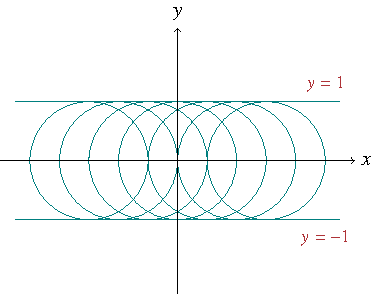
\includegraphics[width=.6\textwidth]{envelope}
\caption{Representation of the family of general solutions of equation \eqref{eq:example-envelope} and its envelopes $y=\pm 1$.}
\label{fig:envelope}
\end{figure}
\end{example}

\begin{example} A classical counterexample to the existence of envelopes is the family of concentric circles at the origin, described by the equation
  \[
  \Phi(x,y,C)=x^2+y^2 -C^2 =0.
  \]
If we tried the usual trick of eliminating $C$ from $\Phi=\Phi_C=0$ we would end up with the equation $x^2+y^2=0$, which in fact is satisfied only by the point $(0,0)$, and thus does not constitute a curve, much less a curve tangent to the family of solutions. A look at Theorem \ref{th:sufficient} tells us that this family does indeed have no envelope, since condition $(iii)$ does not hold at any point. This is also obvious from Figure \ref{fig:concentric}.
\begin{figure}[h!]
\centering
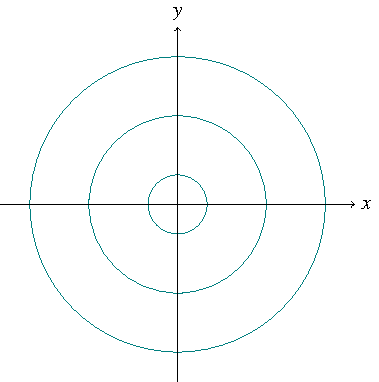
\includegraphics[width=.5\textwidth]{concentric}
\caption{Representation of a family of curves with no envelope.}
\label{fig:concentric}
\end{figure}
\end{example}
